\chapter{Hardware Architecture}
\hspace{10mm}This chapter explains the architecture of the system and the important features of all the components and peripherals used in the system and their significance. This section also talks about the sensors that are part of the BlueBox system. This chapter gives a foundational understanding of the architecture which helps in designing and architecting the firmware.

\section{System overview}
\hspace{10mm} The BlueBox prototype consists of a central board, processor, storage element, microphone, accelerometer and  the environment temperature sensor. The additional electrodes attach to the central board via RS232 interface. The contact microphone attached through a standard 2.5mm audio jack. The body temperature sensor is attached through solder pads in the board. 
The figure \ref{BlueBox_Architecture} shows the overall system architecture for bluebox.
\begin{figure}[h]
	\centering
	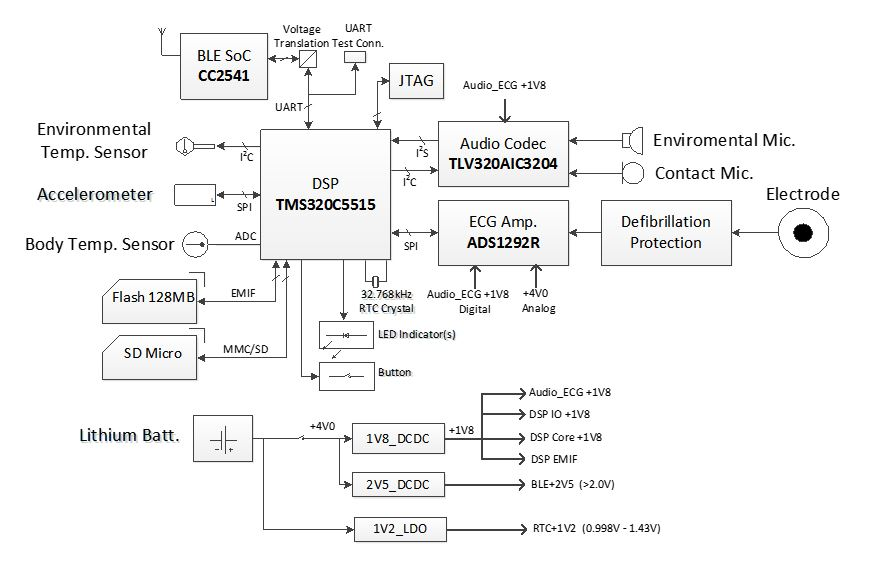
\includegraphics[scale = 0.75 ]{BlueBox_Architecture.JPG}
	\caption{BlueBox Hardware System Architecture\label{BlueBox_Architecture}}
\end{figure} 


\begin{figure}[h]
	\centering
	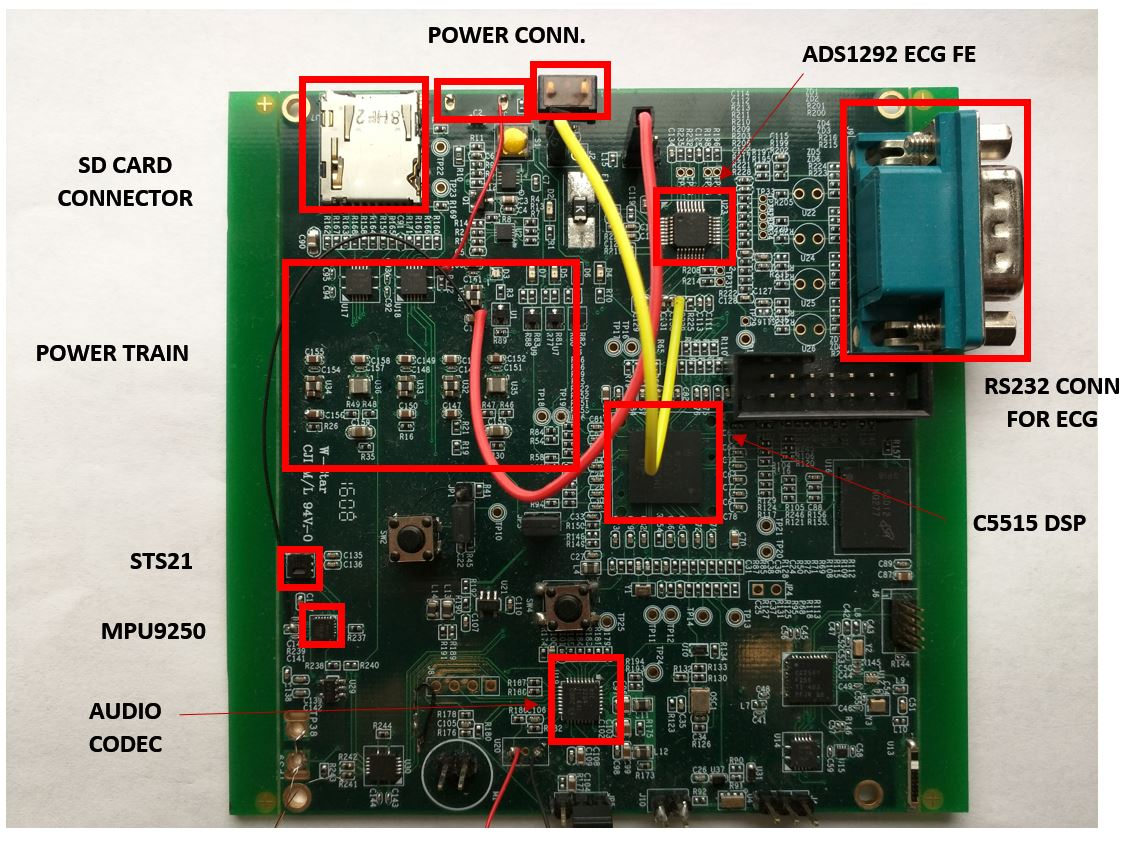
\includegraphics[scale = 0.08]{BlueBox_Hardware.jpg}
	\caption{BlueBox Prototype Hardware \label{BlueBox_Hardware}}
\end{figure} 
\section{Digital Signal Processor}
TMS320C5515 is a fixed-point DSP based on the TMS320C55x™ CPU processor core. The C55x\textsuperscript{TM} DSP architecture achieves high performance and low power through increased parallelism and total focus on power savings. Figure \ref{C5515 Architecture} shows the DSP architecture

\begin{figure}[h]
	\centering
	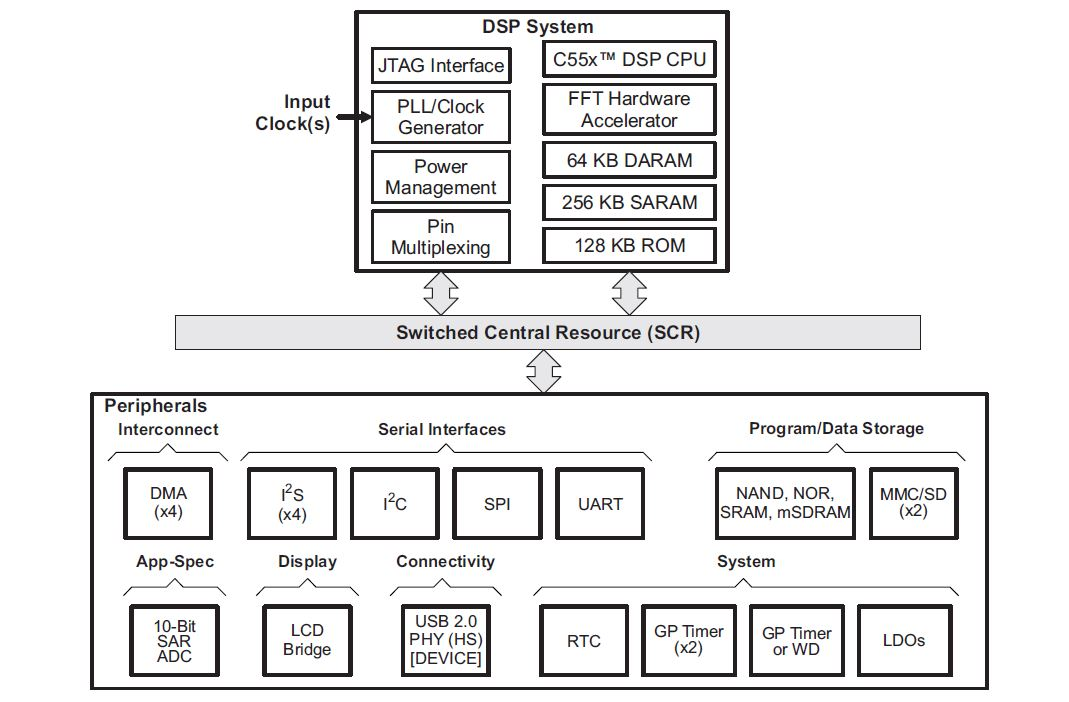
\includegraphics[scale = 0.75 ]{C5515_arch.JPG}
	\caption{DSP Architecture. \cite{tms320c5515}\label{C5515 Architecture}}
\end{figure} 
\subsection{Clock frequency}The DSP has a low power software programmable Phase Locked Loop(PLL) clock generator that  supports 60-,75-,100-,120-MHz clock rate.  
\subsection{On-Chip Memory}The DSP has 320K Bytes Zero-Wait state On-Chip RAM and 128K of On-Chip ROM. 

\subsection{Peripherals} The DSP has general-purpose input and output functions along with the 10-bit SAR ADC provide sufficient pins for status, interrupts, and bit I/O for LCD displays, keyboards, and media interfaces. Serial media is supported through two Multimedia Card/Secure Digital (MMC/SD) peripherals, four Inter-IC Sound (I2S Bus™) modules, one Serial-Port Interface (SPI) with up to 4 chip selects, one I2C multi-master and slave interface, and a Universal Asynchronous Receiver/Transmitter (UART) interface. 

\subsection{DMA} The device includes four Direct Memory Access(DMA) controllers, each with 4 channels, providing data movement for 16-independent channel contexts without CPU intervention. Each DMA controller can perform one 32-bit data transfer per cycle, in parallel and independent of the CPU activity.


\subsection{Power} Furthermore, the device includes three integrated low-droput (LDO) regulators (DSP LDO, ANA LDO, and USB LDO) to power different sections of the device. The DSP LDO can provide 1.3 V or 1.05 V to the DSP core (CVDD), 
selectable on-the-fly by software as long as operating frequency ranges are observed. 


\section{AIC3204 : Audio Codec}
TLV320AIC3204 is an analog interface chip (AIC) of Texas Instruments which is a flexible, low-power, low-voltage stereo audio codec with programmable inputs and outputs, PowerTune capabilities, fixed predefined and parameterizable signal-processing blocks, integrated PLL, integrated LDOs and flexible digital interfaces.  It has both recording and playback capabilities. The record part of the TLV320AIC3204 covers operations from 8kHz mono to 192kHz stereo recording, and contains programmable input channel configurations covering single-ended and differential setups, as well as floating or mixing input signals. It also includes a digitally-controlled stereo microphone preamplifier and integrated microphone bias. It integrates A / D and D / A conversion functions, it achieved high-precision A / D and D / A converter in the low-cost using $\Sigma$-$\Delta$ technology. The size of the chip is very small and compact and its is available in  5 mm × 5 mm 32-pin QFN Package. 

\begin{figure}[h]
	\centering
	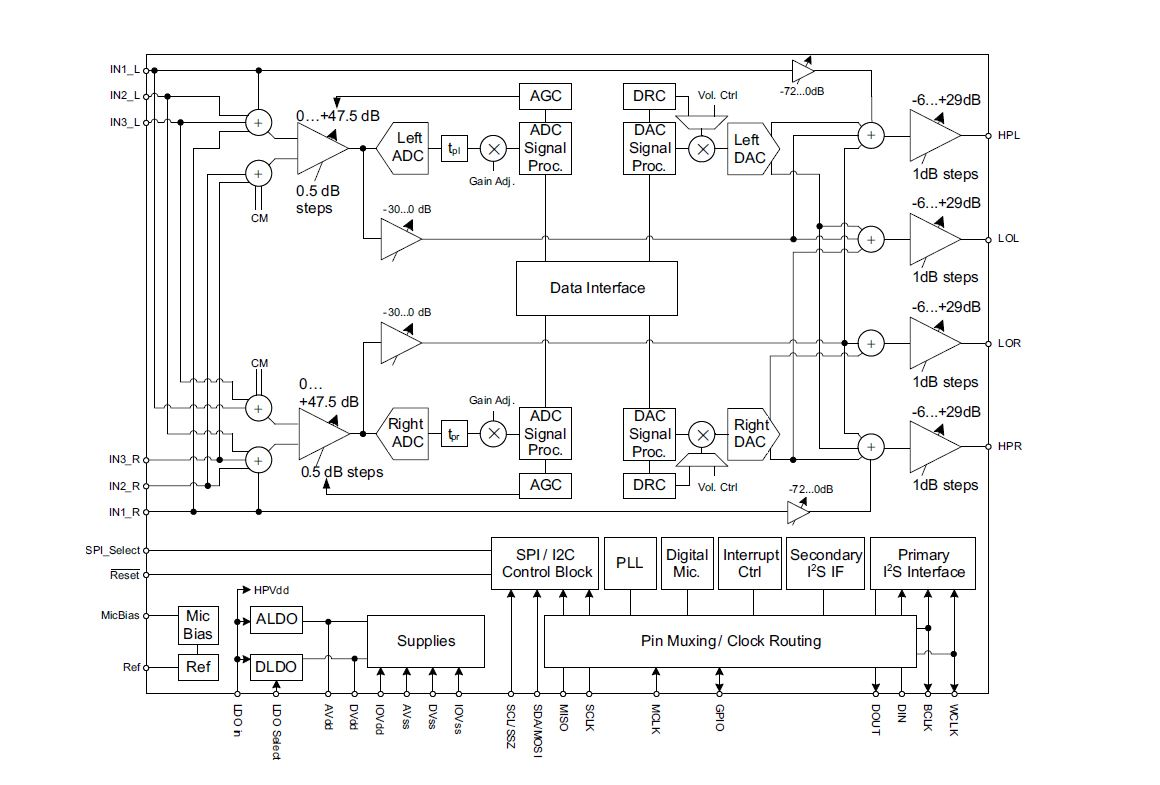
\includegraphics[scale = 0.5 ]{AIC3204.JPG}
	\caption{AIC3204 Block Diagram. \cite{audiocodec}\label{aic3204}}
\end{figure}

Figure \ref{aic3204} displays the audio codec's architecture. It has capabilities of recording stereo audio signals . It has two channels that it can record. One channel is used for respiration recording and the other for paramedic's log recording.
Each
channel of the stereo audio ADC consists of a signal-processing engine with fixed processing blocks.The signal processing blocks available are:
First-order IIR
, Scalable number of biquad filters
, Variable-tap FIR filter
and AGC.The choice between these processing blocks is part of the PowerTune strategy to balance power
conservation and signal-processing flexibility. Less signal-processing capability reduces the power
consumed by the device.
\section{ADS1292R : ECG Frontend}
ADS1292R is the ECG analog front end chip to which the electrode output is connected to.
ADS1292R is a two channel, simultaneous sampling, 24-bit, delta-sigma ($\Delta$$\Sigma$) analog-to-digital converters (ADCs) with a built-in programmable gain amplifier (PGA), internal reference, and an onboard oscillator.  ADS1292R incorporate all features commonly required in portable, low-power medical electrocardiogram (ECG), sports, and fitness applications. With high levels of integration and exceptional performance, the ADS1292R enable the creation of scalable medical instrumentation systems at significantly reduced size, power, and overall cost. ADS1292R have a flexible input multiplexer per channel that can be independently connected to the internally-generated signals for test, temperature, and lead-off detection. Additionally, any configuration of input channels can be selected for derivation of the right leg drive (RLD) output signal. The ADS1292R operate at data rates from 500SPS up to 8 kSPS. The devices are packaged in a 5-mm × 5-mm, 32-pin thin quad flat pack (TQFP). Operating temperature is specified from –40°C to +85°C. ADS1292R is interfaced with the DSP through SPI.
 \begin{figure}[h]
 	\centering
 	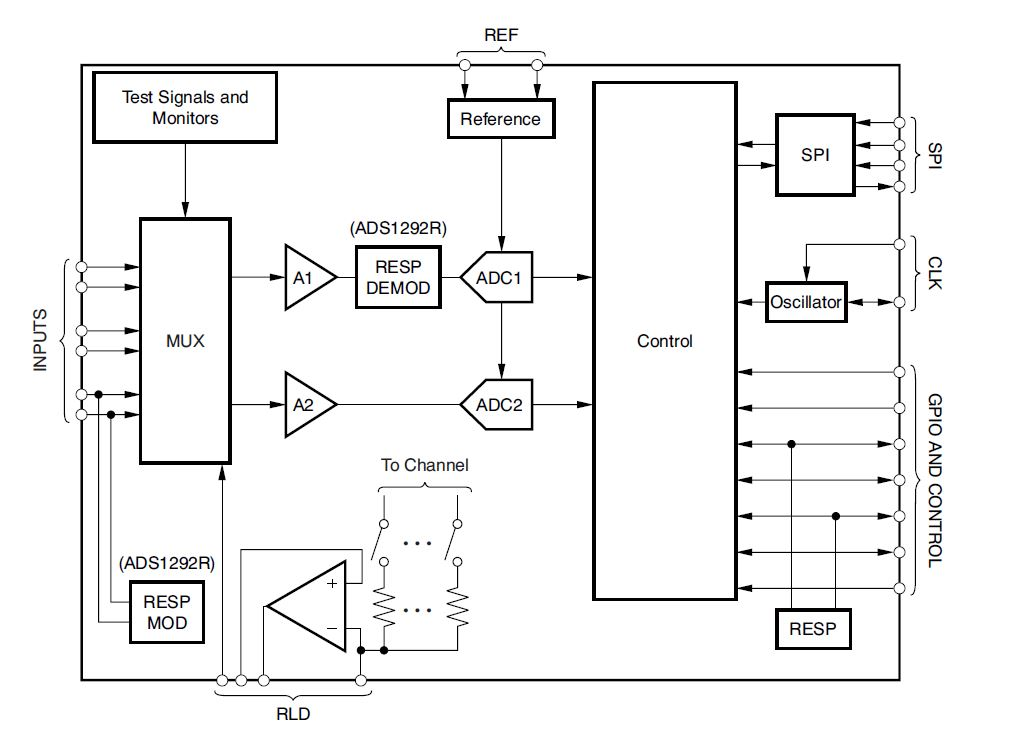
\includegraphics[scale = 0.5 ]{ADS1292R.JPG}
 	\caption{ADS1292R Functional Block Diagram. \cite{ads}\label{ADS1292R}}
 \end{figure}
 
\section{MPU9250 : Accelerometer sensor}\label{mpu9250_def}
MPU-9250 is a 9-axis MotionTracking device that combines a 3-axis gyroscope, 3-axis accelerometer, 3-axis magnetometer and a Digital Motion Processor\textsuperscript{TM} (DMP). With its dedicated I2C sensor bus, the MPU-9250 directly provides complete 9-axis MotionFusion\textsuperscript{TM} output. MPU-9250 features three dedicated 16-bit analog-to-digital converters (ADCs) for digitizing each of the gyroscope outputs, accelerometer outputs, and magnetometer outputs. For precision tracking of both fast and slow motions MPU-9250 provides a user-programmable accelerometer full-scale range of ±2g, ±4g, ±8g, and ±16g. The package size down to a footprint and thickness of 3x3x1mm, to provide a very small yet high performance low cost package. The following figure shows the architecture of MPU9250.A valid accelerometer datat is available 30 ms(typical) after wakeup from sleep.
\begin{figure}[h]
	\centering
	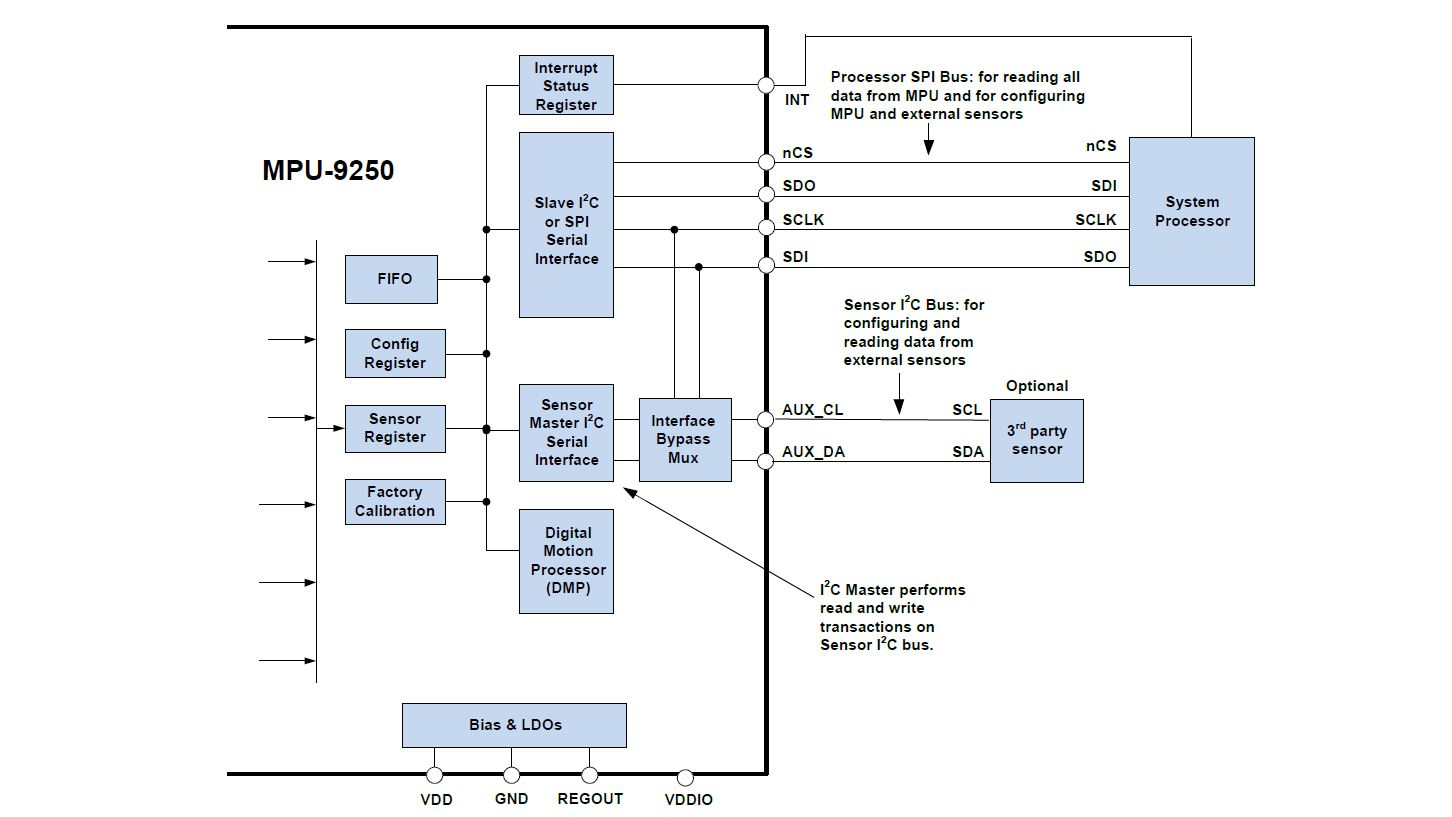
\includegraphics[scale = 0.5 ]{MPU9250.JPG}
	\caption{MPU9250 Architecture. \cite{mpu}\label{mpu9250}}
\end{figure}

The MPU-9250 contains a 512-byte FIFO register that is accessible via the Serial Interface. The FIFO configuration register determines which data is written into the FIFO. Possible choices include gyro data, accelerometer data, temperature readings, auxiliary sensor readings, and FSYNC input. A FIFO counter keeps track of how many bytes of valid data are contained in the FIFO. The FIFO register supports burst reads. The interrupt function may be used to determine when new data is available.

The MPU9250 has multiple user-configurable power modes. The mode which we are interested is Sleep mode (consumes 8 uA)and Low-Power Accelerometer Mode which consumes 450 uA. 
 
\section{Temperature sensor}
\subsection{ STS21 : Environment temperature sensor}
STS21 is a low power, fully self calibrated digital temperature sensor well suited for applications with high demand on temperature accuracy. With dedicated I2C bus it directly provides the temperature output. The sensor comes in a package sized 3 x 3mm footprint and 1.1 mm height. The sensor is powered up to the chosen supply voltage VDD (between 2.1V and 3.6V). After power-up, the sensor needs at most 15ms for reaching idle state, i.e. to be ready accepting commands from the DSP. Current consumption during start up is 350μA maximum. Whenever the sensor is powered up, but not performing a measurement or communicating, it is automatically in sleep mode (idle state). STS21 measures temperature with different resolution ranging from 14 bits to 11 bits, where the 14 bit resolution takes 85ms for conversion whereas a 11 bit resolution takes somewhere between 9 and 11 ms.  

\subsection{MA100: Body temperature sensor} 
MA100 is a Biomedical Chip Thermistor assemblies that are designed for use in applications involving both intermittent and continuous patient temperature monitoring. Although low in cost and small in size, these are highly stable, precision thermochips provide reliability, tight interchangeable tolerances, geometries, and fast response time that are often required.
 
\section{Memory}\label{memory}
The BlueBox system has on-chip memory and the persistent micro SDHC(secure digital high capacity) card storage. Because a micro SD card is power intensive and takes hundreds of milliseconds to write to, the on-chip memory is used as buffer. Once there is enough data in the buffer it is written to the SD card and can be accessed by a computer. All the heavy lifting data transfer are done with the help of Direct Memory access(DMA) peripheral interconnect to take off load from DSP. SD card is interfaced to DSP using MMC/SD interface. The SD card used for the application is a high capacity card that can support a maximum clock frequency of 50 MHz. These high capacity cards are not byte addressable. They are organized in 512 Byte sector or block and thus are block addressable. BlueBox uses kingston 8 GB micro SDHC card. the SDHC card is very power hungry. It consumes 150 mA  when operated at 50 MHz  during active read/write operation and consumes 30 mA during inactive periods.

\section{Battery and Power management circuitry}
 A GMB 302547 Lithium ion polymer rechargable battery, shown in figure \ref{fig:battery} is used to power the system. It has a capacity of 300 mAH at 3.7 V. It is 4 cm long , 2cm wide and 0.2 mm thick. And it weighs  8 grams. The battery is place on top of the central board housing. The central board has a battery charging circuitry that can charge the battery completely in 2 hours. The power management circuitry provides a power-train that feeds the different power domain of the DSP  as shown figure \ref{BlueBox_Architecture}.    
 \begin{figure}[h]
 	\centering
 	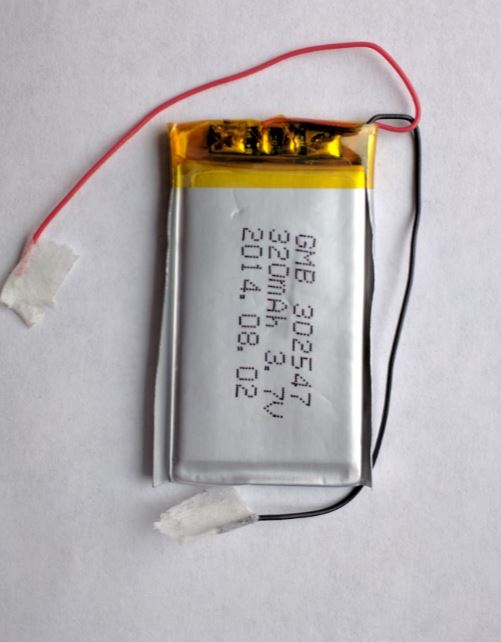
\includegraphics[scale = 0.5 ]{battery.JPG}
 	\caption{Lithium Polymer battery}\label{fig:battery}
 \end{figure}       
%%% Local Variables: ***
%%% mode: latex ***
%%% TeX-master: "thesis.tex" ***
%%% End: ***
